\section{Performance Evaluation} \label{sec:performance-evaluation}

\subsection{Objectives} \label{subsec:objectives}

Our trajectory planner aims to minimize a cost function that represents the driving behavior we desire.
The cost function is composed of several objectives, each weighted by a corresponding factor.

The primary objectives considered are control effort, deviation from the reference trajectory, and terminal state accuracy.
The control effort objective aims to minimize
the numerical derivatives of control inputs to ensure smooth driving, represented by the cost function:
\begin{equation}
	J_{control} = \sum_{i=0}^{n-1} \left\| d_1(t_i) \right\|^2
\end{equation}
where $d_1(t_i)\in \mathbb{R}^{dim(u)}$ is an auxiliary variable constrained by: \[
	d_1(t_i) = \frac{u(t_i) - u(t_{i-1})}{t_i - t_{i-1}}
\]

The tracking objective aims to minimize the deviation from the center of the road, represented by the cost function:
\begin{equation}
	J_{tracking} = \sum_{i=0}^{n} d_2(t_i)^2
\end{equation}
where $d_2(t_i)\in \mathbb{R}$ is an auxiliary variable constrained by: \[
	0 \leq d_2(t_i) \leq \min \left\{ \overline{n}(s(t_i)) - n(t_i), n(t_i) - \underline{n}(s(t_i)) \right\}
\]

The terminal state objective aims to minimize the deviation from a desired terminal state $x_{final}$ at the final time step $t_n$, represented by the cost function:
\begin{equation}
	J_{terminal} = \|x(t_n) - x_{final}\|^2
\end{equation}

The total cost function $J$ is a weighted sum of these objectives:
\begin{equation}
	J = \alpha J_{control} + \beta J_{tracking} + \gamma J_{terminal} \end{equation} where $\alpha$, $\beta$, and $\gamma$ are the weights that determine
the relative importance of each objective.
By minimizing this cost function, our trajectory planner generates a trajectory that balances control effort, tracking the reference trajectory, and
accuracy in reaching the desired terminal state.

\subsection{Scenarios} \label{subsec:scenarios}

In order to evaluate the performance of our trajectory planner, we implemented several driving scenarios.
These scenarios are designed to test different aspects of the planner's capabilities.
The Straight Road scenario evaluates the planner's ability to maintain a straight path with minimal control effort, ensuring smooth and efficient
driving.
In the Left Turn scenario, the planner's performance is assessed based on its ability to execute a smooth left turn while adhering to the reference
trajectory.
The Lane Change scenario tests the planner's capability to perform a lane change maneuver safely and efficiently, highlighting its responsiveness and
precision.
The Slalom scenario challenges the planner to navigate through a series of closely spaced obstacles, requiring precise control and smooth transitions
between maneuvers.
The Elchtest, also known as the moose test, evaluates the planner's ability to perform a sudden evasive maneuver to avoid an obstacle, testing its
quick decision-making and control under pressure.
The Elchtest scenario can be visualized as follows:
\begin{figure}[H]
	\centering
	\begin{tikzpicture}
		\draw[thick, dashed] (0,-0.5) -- (5,-0.5); % Road boundary
		\draw[thick, dashed] (0,0.5) -- (3,0.5); % Road boundary
		\draw[thick, dashed] (3,0.5) -- (3,1.5); % Road boundary
		\draw[thick, dashed] (5,0.5) -- (5,-0.5); % Road boundary
		\draw[thick, dashed] (5,0.5) -- (7,0.5); % Road boundary
		\draw[thick, dashed] (3,1.5) -- (9,1.5); % Road boundary
		\draw[thick, dashed] (9,0.5) -- (9,1.5); % Road boundary
		\draw[thick, dashed] (7,0.5) -- (7,-0.5); % Road boundary
		\draw[thick, dashed] (7,-0.5) -- (12,-0.5); % Road boundary
		\draw[thick, dashed] (9,0.5) -- (12,0.5); % Road boundary
		\node at (0,0) {Start};
		\node at (12,0) {End};
	\end{tikzpicture}
	\caption{Elchtest scenario visualization}
	\label{fig:elchtest}
\end{figure}

Finally, the Sharp U Turn scenario tests the planner's ability to execute a sharp U-turn, challenging its control effort and adherence to the desired
terminal state.

By evaluating the planner in these diverse scenarios, we can gain a comprehensive understanding of its strengths and areas for improvement.

\begin{longtable}{l c c c c c}
	\caption{Overview of Road Segments and Their Properties}                                                                                             \\
	\toprule
	\textbf{Road Name}                & \textbf{Segment} & \textbf{Length} & \textbf{Curvature} & \multicolumn{2}{c}{\textbf{Lane Width}}                \\
	\cmidrule(lr){5-6}
	                                  &                  &                 &                    & \textbf{Start}                          & \textbf{End} \\
	\midrule
	\endfirsthead

	\multicolumn{6}{c}{\textit{Continued from previous page}}                                                                                            \\
	\toprule
	\textbf{Road Name}                & \textbf{Segment} & \textbf{Length} & \textbf{Curvature} & \multicolumn{2}{c}{\textbf{Lane Width}}                \\
	\cmidrule(lr){5-6}
	                                  &                  &                 &                    & \textbf{Start}                          & \textbf{End} \\
	\midrule
	\endhead

	\bottomrule
	\multicolumn{6}{c}{\textit{Continued on next page}}                                                                                                  \\
	\endfoot

	\bottomrule
	\endlastfoot

	\multirow{5}{*}{Elchtest}         & 1                & 12.0            & 0.000              & [-1.0,1.0]                              & [-1.0,1.0]   \\
	                                  & 2                & 13.5            & 0.000              & [-1.0,1.0]                              & [2.0,4.7]    \\
	                                  & 3                & 11.0            & 0.000              & [2.0,4.7]                               & [2.0,4.7]    \\
	                                  & 4                & 12.5            & 0.000              & [2.0,4.7]                               & [-1.0,1.0]   \\
	                                  & 5                & 12.0            & 0.000              & [-1.0,1.0]                              & [-1.0,1.0]   \\
	\midrule
	\multirow{1}{*}{Left Turn}        & 1                & 235.6           & 0.007              & [-2.0,2.0]                              & [-2.0,2.0]   \\
	\midrule
	\multirow{1}{*}{Straight}         & 1                & 180.0           & 0.000              & [-2.0,2.0]                              & [-2.0,2.0]   \\
	\midrule
	\multirow{4}{*}{Lane Change}      & 1                & 30.0            & 0.000              & [-2.0,2.0]                              & [-2.0,2.0]   \\
	                                  & 2                & 20.9            & 0.025              & [-2.0,2.0]                              & [-2.0,2.0]   \\
	                                  & 3                & 20.9            & -0.025             & [-2.0,2.0]                              & [-2.0,2.0]   \\
	                                  & 4                & 30.0            & 0.000              & [-2.0,2.0]                              & [-2.0,2.0]   \\
	\midrule
	\multirow{5}{*}{Slalom}           & 1                & 20.0            & 0.000              & [-2.0,2.0]                              & [-2.0,2.0]   \\
	                                  & 2                & 94.2            & -0.033             & [-2.0,2.0]                              & [-2.0,2.0]   \\
	                                  & 3                & 94.2            & 0.033              & [-2.0,2.0]                              & [-2.0,2.0]   \\
	                                  & 4                & 94.2            & -0.033             & [-2.0,2.0]                              & [-2.0,2.0]   \\
	                                  & 5                & 20.0            & 0.000              & [-2.0,2.0]                              & [-2.0,2.0]   \\
	\midrule
	\multirow{3}{*}{Feasible Curve}   & 1                & 20.0            & 0.000              & [-2.0,2.0]                              & [-2.0,2.0]   \\
	                                  & 2                & 15.7            & 0.200              & [-2.0,2.0]                              & [-2.0,2.0]   \\
	                                  & 3                & 20.0            & 0.000              & [-2.0,2.0]                              & [-2.0,2.0]   \\
	\midrule
	\multirow{3}{*}{Infeasible Curve} & 1                & 20.0            & 0.000              & [-2.0,2.0]                              & [-2.0,2.0]   \\
	                                  & 2                & 8.8             & 0.357              & [-2.0,2.0]                              & [-2.0,2.0]   \\
	                                  & 3                & 20.0            & 0.000              & [-2.0,2.0]                              & [-2.0,2.0]   \\
	\midrule
\end{longtable}

\subsection{Simulation Setup} \label{subsec:simulation}

For the vehicle simulation, we employ a more sophisticated model and discretize its dynamics using the Runge-Kutta method, which offers greater
accuracy compared to the forward Euler method used for trajectory planning.
To ensure reproducibility, we define the model using the following state variables and control inputs: \[ x = [p_x, p_y, \delta, v, \psi, \dot{\psi},
	\beta]^T, u = [a_x, v_{\delta}]^T \] where $p_x$, $p_y$ represent the vehicle's position coordinates, $\delta$ is the steering angle, $v$ is the
velocity, $\psi$ is the yaw angle, $\dot{\psi}$ is the yaw rate, $\beta$ is the slip angle, $a_x$ is the longitudinal acceleration, and $v_\delta$ is
the steering rate.

The model's dynamics are governed by the following equations, valid for $|v|\geq0.1$:
\[
	f(x, u) = \begin{bmatrix}
		v\cos(\psi + \beta)                                  \\
		v\sin(\psi + \beta)                                  \\
		v_\delta                                             \\
		a_x                                                  \\
		\dot{\psi}                                           \\
		\frac{\mu\,m}{I_{z}(l_{r}+l_{f})}\Bigl(
		l_{f}\,C_{S,f}\bigl(g\,l_{r}-a_xh_{cg}\bigr)\,\delta \\
		\;+                                                 \;\bigl[l_{r}\,C_{S,r}\bigl(g\,l_{f}+a_xh_{cg}\bigr)
			\;-\;l_{f}\,C_{S,f}\bigl(g\,l_{r}-a_xh_{cg}\bigr)\bigr]\,\beta
		\Bigr)                                               \\
		\quad -\;\Bigl[
		l_{f}^{2}\,C_{S,f}\bigl(g\,l_{r}-a_xh_{cg}\bigr)
		\;+\;
		l_{r}^{2}\,C_{S,r}\bigl(g\,l_{f}+a_xh_{cg}\bigr)
		\Bigr]
		\frac{\dot{\psi}}{v}                                 \\
		\frac{\mu}{v\,\bigl(l_{r}+l_{f}\bigr)}\Bigl(
		C_{S,f}\bigl(g\,l_{r}-a_xh_{cg}\bigr)\,\delta
		\;-\;
		\bigl[C_{S,r}\bigl(g\,l_{f}+a_xh_{cg}\bigr)          \\
			\;+\;
		C_{S,f}\bigl(g\,l_{r}-a_xh_{cg}\bigr)\bigr]\,\beta   \\
		\quad +\;\bigl[
			C_{S,r}\bigl(g\,l_{f}+a_xh_{cg}\bigr)\,l_{r}
			\;-\;
			C_{S,f}\bigl(g\,l_{r}-a_xh_{cg}\bigr)\,l_{f}
			\bigr]
		\frac{\dot{\psi}}{v}
		\Bigr)
		\;-\;
		\dot{\psi}
	\end{bmatrix}
\]
For smaller velocities $|v|<0.1$, the dynamics simplify to:
\[
	f(x, u) = \begin{bmatrix}
		v\cos(\psi + \beta) \\
		v\sin(\psi + \beta) \\
		v_\delta            \\
		a_x                 \\
		\dot{\psi}          \\
		\frac{1}{l_{wb}}
		\biggl(
		a_x\,\cos( \beta)\,\tan(\delta)
		\;-\;
		v\,\sin( \beta)\,\tan(\delta)\,\dot{x}_{7}
		\;+\;
		\frac{v\,\cos( \beta)}{\cos^2(\delta)}\,
		v_{\delta}
		\biggr)
		\\
		\frac{1}{1 +
			\bigl(\tan(\delta)\tfrac{l_{r}}{l_{wb}}\bigr)^2}
		\;\cdot\;
		\frac{l_{r}}{l_{wb}\,\cos^2(\delta)}\,
		v_{\delta}
	\end{bmatrix}
\]

We consider a vehicle of length \(l = 4.298\,\mathrm{m}\) and width \(w = 1.674\,\mathrm{m}\), with total mass \(m = 1.225\times10^3\,\mathrm{kg}\)
and moment of inertia \(I_z = 1.538\times10^3\,\mathrm{kg\,m}^2\).
The center of gravity is located \(l_f = 0.883\,\mathrm{m}\) from the front axle and \(l_r = 1.508\,\mathrm{m}\) from the rear axle, at a height
\(h_{cg} = 0.557\,\mathrm{m}\).
The front and rear cornering stiffness coefficients are both \(C_{S,f} = C_{S,r} = 20.89\,\text{[1/rad]}\), and the friction coefficient is \(\mu =
1.048\).

\subsubsection{Replanning Strategy}

In our simulation, we employed a replanning strategy to implement a feedback mechanism.
In addition to the time horizon, we implemented a fixed time interval, shorter than the time horizon, after which the planner recalculates the
trajectory from the current position of the vehicle.
This replanning mechanism allows the planner to adjust to changes in the environment or deviations from the planned path.
We employed a time discretization of equal intervals for the replanning time interval, and the time intervals increase linearly for the remaining
time horizon.

\begin{figure}[h]
	\centering
	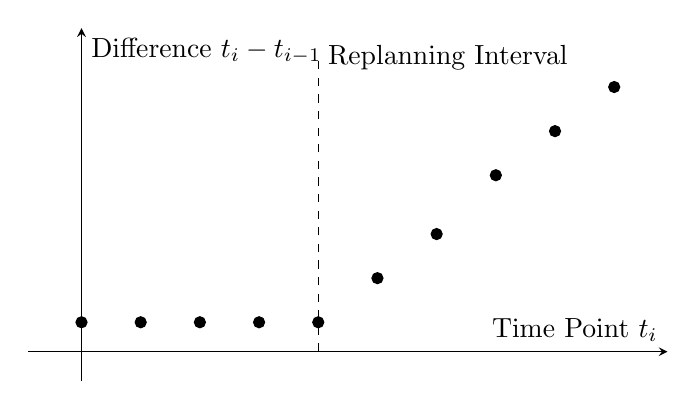
\begin{tikzpicture}
		\begin{axis}[
				xlabel={Time Point $t_i$},
				ylabel={Difference $t_i - t_{i-1}$},
				width=0.8\textwidth,
				height=0.5\textwidth,
				grid=major,
				axis lines=middle,
				enlargelimits=true,
				xtick=\empty, % Remove x-axis ticks
				ytick=\empty, % Remove y-axis ticks
				clip=false
			]
			% Data points
			\addplot[only marks, mark=*, mark size=2pt]
			coordinates {
					(0,0.2) (1,0.2) (2,0.2) (3,0.2) (4,0.2) (5,0.5) (6,0.8) (7,1.2) (8,1.5) (9,1.8)
				};

			% Dashed vertical line for replanning interval
			\addplot[dashed] coordinates {(4,0) (4,2)};

			% Replanning label
			\node[anchor=west] at (axis cs:4,2) {Replanning Interval};

		\end{axis}
	\end{tikzpicture}
	\caption{Time points and their differences to previous time points}
	\label{fig:time_points}
\end{figure}

Figure \ref{fig:time_points} illustrates the time points and their intervals.
The states for the time points to the left of the dashed line are simulated, after which a replanning is triggered.
This replanning follows the same time discretization pattern as the initial planning phase.
The term $\Delta t$ refers to the time intervals between the initial time points, which vary across the different benchmark scenarios.
The slope of time difference after the replanning interval is given by $\Delta^2 t_{replan}$.

\subsection{Results}
\label{subsec:results}

\subsection*{Point Mass Model}

\paragraph{Assumptions and Simplifications.}
The point mass model simplifies the vehicle to a single mass concentrated at a point.
It assumes that the path is primarily driven by the longitudinal and lateral accelerations as constrained by the road alignment.
Key kinematic effects such as tire slip angles, lateral load transfer, or steering geometry are either omitted or treated in a highly simplified
manner.
Furthermore, it often assumes that the orientation of the mass aligns with the road direction, so the model is well suited for higher-level path
planning over a known trajectory, where the exact wheel and steering configuration are less critical.

\paragraph{Performance Characteristics.}
Because of its simpler nature, the point mass model generally offers:
\begin{itemize}
	\item \textbf{Lower computational cost}, enabling faster simulations and
	      easier real-time implementation for basic path tracking.
	\item \textbf{Reduced parameter dependency}, as it needs fewer vehicle
	      parameters (e.g., just mass and approximate friction limits).
	\item \textbf{Reduced accuracy in nonlinear conditions}, because it neglects
	      steering geometry, tire slip angles, and more nuanced lateral
	      dynamics---making it less accurate at high lateral accelerations
	      or large steering angles.
\end{itemize}

\subsection*{Kinematic Bicycle Model}

\paragraph{Assumptions and Structure.}
The kinematic bicycle model represents the vehicle by a single front tire and rear tire, capturing the geometric relationship among steering angle,
vehicle length, and lateral motion.
It models the steering input at the front axle while assuming no explicit slip at the tire contact patch (although slip angles may be implicitly
captured via kinematic relations).
Unlike a full dynamic model, it generally omits complex tire forces and weight transfer, but retains essential geometry required to describe the
vehicle’s heading and turning radius accurately

\paragraph{Performance Characteristics.
}
Compared to the point mass model, the kinematic bicycle model typically has:
\begin{itemize}
	\item \textbf{Improved representation of vehicle posture}, because it
	      tracks yaw angle and the relation between front and rear axle motions.
	\item \textbf{Better handling of moderate steering maneuvers}, as it
	      can capture how steering inputs alter the effective turning radius
	      and orientation.
	\item \textbf{Moderate computational complexity}, still significantly
	      lighter than full dynamic models but more detailed than
	      a point mass approach.
	\item \textbf{Limitations at high speeds or extreme maneuvers}, as it
	      ignores tire slip forces and load transfers, thus limiting
	      predictive capability in aggressive cornering or low-adhesion
	      conditions.
\end{itemize}